\documentclass[12pt, a4paper]{article}
\usepackage{graphicx}
\graphicspath{ {images/} }
\usepackage{amsmath} % many things
\usepackage{physics} % (partial) derivatives, etc.
\usepackage{siunitx}
\usepackage{hyperref}
\hypersetup{
    colorlinks=true,
    linkcolor=black,
    filecolor=black,
    urlcolor=blue,
    citecolor=black,
}
\usepackage{amssymb}
\usepackage{subfigure}



\let\oldexp\exp
\renewcommand{\exp}[1]{\ensuremath{\oldexp \left( #1 \right)}}
%\renewcommand{\exp}[1]{\ensuremath{\left(#1\right)}}

\textwidth=170mm
\textheight=250mm
\hoffset= -20mm       % may need change
\voffset= -25mm       % may need change

\begin{document}
%% we create our own title page
\thispagestyle{empty}     % only for frontpage
\null\vspace{40mm}
\begin{center}
{%%%%%%%%%%%%%%%%%%%%%%%%%% Title
\Large  Magneto-Optical Trap
\footnote{\noindent Experiment F20, performed on 26\textsuperscript{th} August 2019,
Supervisor Saba Zia Hassan,
short special evaluation}
}\\[15mm]
%%%%%%%%%%%%%%%%%%%%%%%%%%% Authors
L. Hahn and L. Kuehmichel

\vspace{25mm}

\parbox{0.9\textwidth}{
Abstract:\\\\   
\small In this experiment, we used a MOT to analyze the absorptive spectra of Rubidium atoms, including the fine and hyperfine energy level splittings. We then used laser cooling and looked at how quickly atoms escape the trap in order to determine how low we could cool the gas.
\\\\
We determined a natural line width of $\approx 6 \si{\mega\hertz}$ as well as relatively accurate hyperfine separation levels, compared with their respective literature values. The temperature of the Rubidium gas during laser cooling was lowest with a detuning of $\approx -8.5 \si{\mega\hertz}$, where it dropped to several hundred $\si{\micro\kelvin}$.
}
\end{center}

\vfill
Audited as a special evaluation: Date, Signature:
\vspace{20mm}

%% Empty backside of title page, remove for single-sided printing
% \newpage  
\null\thispagestyle{empty} 
   
%\newpage
%\tableofcontents 

\newpage

\pagenumbering{arabic} %% start page 1 
\section{Introduction: Physical Subjects and Goal of the Experiment}
\subsection{Basic Overview of Physical Subjects}
The Magneto-Opitcal Trap makes use of an abundance of physical topics mainly focussed around atomic pyhsics, optics and spectroscopy. The following section aims to provide an overview of these topics without an in-depth explanation. The source of all the information summarised in Chapter 1 is \cite{script}, where one can find more in-depth information on the subject.
\subsubsection{Level Structure of Rubidium Atoms and Laser Spectroscopy}
\begin{figure}
    \centering
    \parbox{0.4\textwidth}{
        \centering
        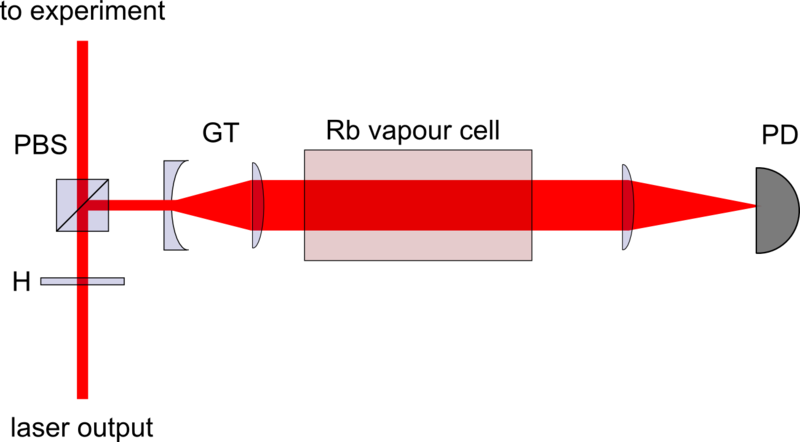
\includegraphics[width=0.4\textwidth]{800px-Doppler_spectroscopy.png}
    }

    \caption{Schematic sketch of the spectroscopy path with:  PBS being a polarizing beam splitter, GT means Galilean Telescope and H references a half waveplate, \cite{script}}
    \label{doppler_spect}
\end{figure}

As shown in Fig.\ref{doppler_spect}, the laser beam passes a Rb vapour cell before hitting a photo diode, where the intensity is evaluated. Simultaneously, the laser scans through various frequencies to measure an intensity response. As the laser propagates through the gas, the stimulated atomic state transitions have an effect on the laser intensity following the Lambert-Beer law:
\begin{equation}
\frac{dI}{dx}= -\kappa I
\end{equation}
where $\kappa = h\nu n_0 \alpha (P_0 - P_1)$ denotes the absorption coefficient, $x$ the path and $I$ the beam intensity. Furthermore:
\begin{equation}
\alpha = \alpha_0 \mathcal{L}(\nu , \nu_0)
\end{equation}
describes the frequency dependence of $\kappa$, which has a Lorentzian shape. The expression $P_0 - P_1$ gives us the relation between atoms in the excited ($P_1$) versus the ground state ($P_0$). The fraction $\frac{P_1}{P_0}$ has a Gaussian shape and depends on frequency and temperature.
A complication for evaluating the exact position of absorption dips are the Doppler shifts created through the movement of the atoms in the vapour cell. The so-called "Doppler broadening" which we then can observe in our Intensity-Frequency-diagram has a Gaussian shape with the standard deviation being:
\begin{equation}
\sigma_v = \sqrt{\frac{k_B T}{m}}
\end{equation}
where $T$ denotes the temperature, $k_B$ the Boltzmann constant and $m$ the mass of a particle. Through all these considerations, we can then describe the different populations of $P_0$ and $P_1$ accordingly and arrive at the Doppler free spectroscopy: instead of using one single beam, we use a probing beam and a pumping beam which are detuned in the order of a few Megahertz to evaluate the Doppler shift dependeny. The interplay of these two beams creates a so-called "saturated absorption dip" right at the resonance frequency without doppler shifting but depends on $\frac{I}{I_{sat}}$ with $I_{sat}$ being the saturation intensity, which depends on spontaneous emission rate of the atoms and $\alpha$.

\begin{figure}
    \centering
    \parbox{0.4\textwidth}{
        \centering
        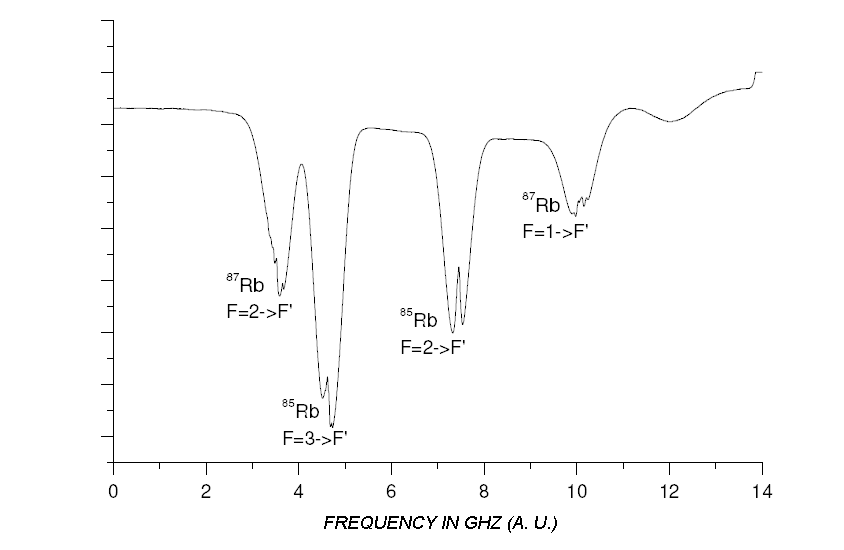
\includegraphics[width=0.4\textwidth]{Rb_satabs.png}
    }

    \caption{measured spectra with cross-over resonances, \cite{script}}
    \label{measured_spec}
\end{figure}

Since the Rubidium atoms have a more complicated V-shaped energy level schematic (two upper energy levels and one lower), the process creates crossover-peaks which can be observed in the Gaussian absorption dip.
Rubidium has fine structure levels with L-S coupling
\begin{equation}
\vec{J} = \vec{L} + \vec{S}
\end{equation}
($\vec{J}$ = total electronic angular momentum, $\vec{L}$ = total orbital angular momentum, $\vec{S}$ = total electronic spin angular momentum)

and hyperfine structure levels with I-J coupling
\begin{equation}
\vec{F} = \vec{I} + \vec{J}
\end{equation}
($\vec{F}$ = total angular momentum, $\vec{I}$ = spin angular momentum)
which complicate the doppler-free absorption spectrum even further.
All these effects can be seen in accumulation in Fig.\ref{measured_spec}

Also, we make use of frequency modulation spectroscopy in order to measure the Lamb-dips and cross-overs as well as to stabilise the laser in the MOT-part of the experiment. Through a series of effects, one gets a derivative of the absorption signal and therefore can estimate the position of the absorption dip more accurately. This whole process is done in the spectroscopy-branch of the experimental setup. \cite{script}

\subsubsection{Magneto-Optical Trap}
The Magneto-Optical trap used to cool atoms to a few $100\ \mu  K$ uses two main principles: the effect of optical molasses and the Zeeman-effect, which occurs under the influence of an external magetic field gradient. The linear momentum imposed upon atoms by light can be written as $p=\hbar k$. Furthermore $\hbar \omega$ changes the internal energy of an atom and the angular momentum has effect on the orbital angular momentum $l$ with the selection rule $\Delta l=\pm 1$. Through these elementary processes, the atoms are slowed down in the optical molasses (OM): two opposing standing-wave laser beams dampen the atomic motion where the force $\vec{F}_{OM}$ is proportional to the velocity of the atoms $-\vec{v}$. This process only works in cooperation with the doppler-free spectroscopy, since the resonance frequencies must be "scanned" and acquired.

However, there are limits to cooling via OM: the recoil limit (for $^{85}Rb$, $T_r = 0.370\mu K$) and doppler temperature limit (for $^{85}Rb$, $T_D = 143.41\mu K$), which limit the cooling to a few hundreds of $\mu K$.

The MOT is comosed of a quadrupole magnetic field and three pairs of counter propagating laser beams.
The actual trapping is achieved through a anti-Helmholtz-coil, which makes use of the $M_e$-Zeeman-component-splitting to $M_e = +1$ and $M_e = -1$ depending on the polarisation of the light and to which direction the atoms are escaping.

The missing link between measuring the temperature of our MOT and the physics mentioned above is the so called "release-recapture method" which has as its base the rate equation:
\begin{equation}
\frac{dN}{dt} = L - \alpha N
\end{equation}
where $N$ denotes the number of trapped particles, $L$ the loss-rate and $\alpha$ the one-body loss coefficient. The solution is given by:
\begin{equation}
N(t) = \frac{L}{\alpha}(1-e^{-\alpha x})
\end{equation}
Later, the laser is switched on and off to analise the number of recaptured atoms $N(t)$ after a varying time interval, in which the laser is turned off.
Through the Stefan-Boltzmann velocity distribution, one arrives at the follwing fraction in order to compute the temperature $T$:
\begin{equation}
\frac{N(t)}{N(0)} = erf(\chi) - \frac{2}{\sqrt{\pi}} \chi e^{-\chi ^2}
\end{equation}
where $\chi = \sqrt{\frac{M}{k_{b} T}}\frac{R}{t}$, $t$ is the time stamp at which MOT is turned back on, $N(0)$ is the initial atom number (where the trap is fully loaded), $M$ is the particle mass and $R=1.5$mm the radius of the atom cloud. \cite{script}


\subsection{Goal of the Experiment}
The goal of the experiment is to analise doppler-free spectra and match atomic transitions to dips in our measurements as well as to calculate the MOT-temperature with the trap turned off. In the second part of the experiment we acquire $\alpha$ and $L$ in dependency of different detuning frequencies and Helmholtz-coil currents in order to generate the parameters which maximise the number of trapped atoms. Then, through a release-recapture measurement, we calculate the temperature of the MOT.


\section{Experimental Setup}

\begin{figure}[h]
\centering
    \subfigure[MOT setup]{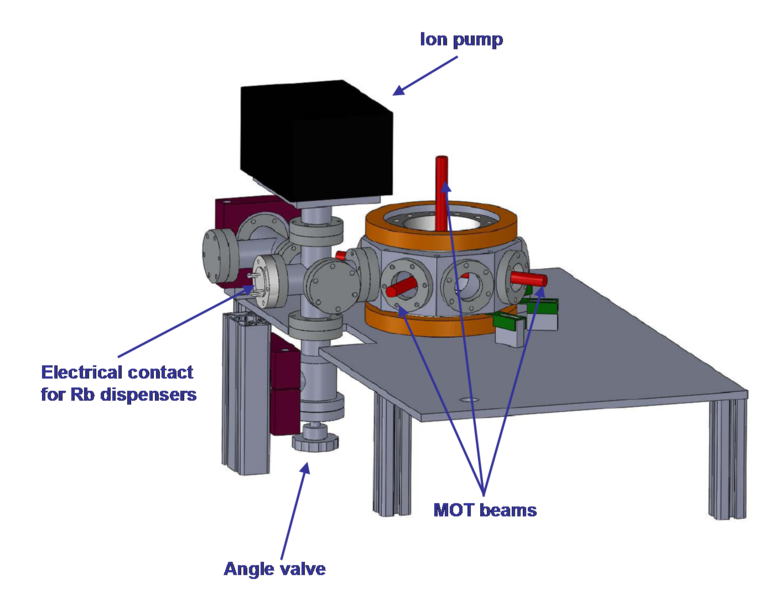
\includegraphics[width=0.35\textwidth]{779px-Vacuum_chamber_2.png}}
    \subfigure[optical setup]{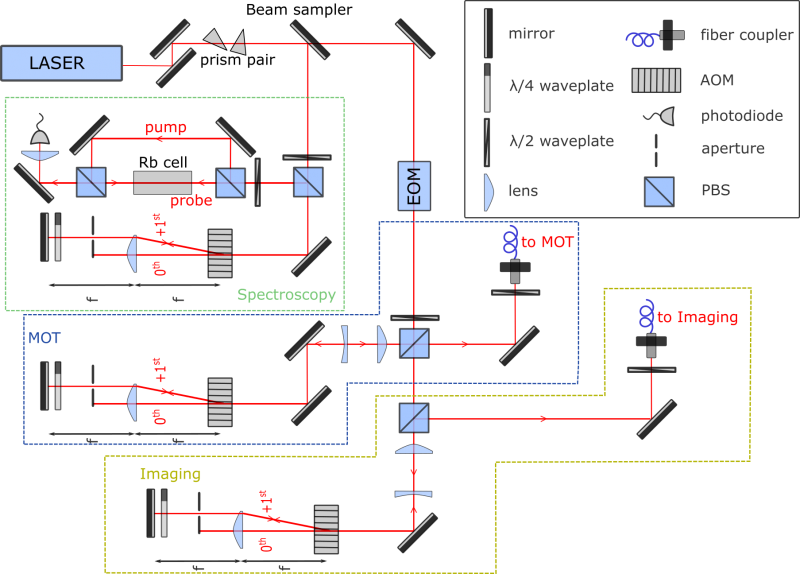
\includegraphics[width=0.35\textwidth]{800px-Setup-schematic.png}}
\caption{Schematics of the experimental setup, \cite{script}}
	\label{expsetup}
\end{figure}

\subsection{Diode lasers and laser locking}
This experiment is equipped with two home-built external cavity diode lasers for addressing the cooling transition and the repumping transition. The frequency of both lasers can be altered with an in-built acousto-optic modulator (AOM). The piezo crystal, which generates the AOM, can be influenced by changing the offset voltage on the controller (Thorlabs MDT693A).

In order to stabilise the laser signal (no fluctuations in intensity and frequency), we make use of a digital PID controller (Toptica Digilock 110). This device was also used to change the detuning of the two laser beams by adjusting a screw on the front panel of the device.

These devices allow for a laser accuracy of 1MHz, which is less than the natural linewidth of the atomic transition.

\subsection{Optical setup}
The optical setup is presented in Fig. 3 (b) and roughly consist of a spectroscopy path, a MOT path and an imaging path. We make use of anamorphic prism pairs, optical isolators, wave plates, beam splitters, a laser beam expansion, AOMs, photo diodes and a double pass configuration (for the AOM).

\subsection{Vacuum system}
The vacuum system is shown in Fig. 3 (a). It consist the vacuum sealed housing itself, of an ion pump, an anti-Helmholtz coil and windows for the six laser beams. With the ion pump, we create an ultra-high vacuum (UHV) environment of about $10^{-9}$ mbar, without which the experiment would fail due to collisions with air molecules. The anti-Helmholtz coils have a diameter of about 170 mm and a distance of 115 mm. They can sustain currents of up to 11A.

\section{Measured Data}
\begin{figure}[h]
\centering
    \subfigure[example of a loading curve captured with an oscilloscope]{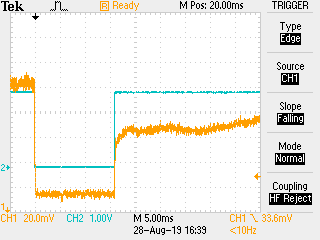
\includegraphics[width=0.3\textwidth]{F0020TEK.png}}
    \subfigure[the full raw spectrum with the derivative visible]{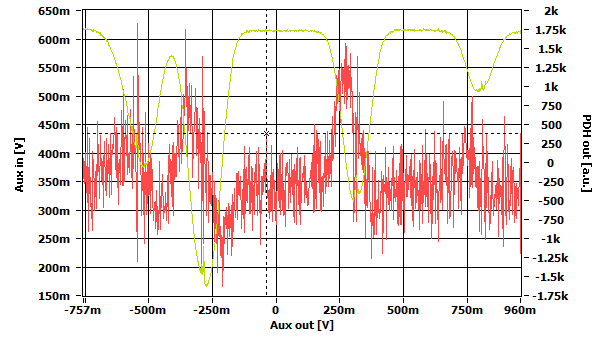
\includegraphics[width=0.41\textwidth]{fullspectrum_meas.png}}
\caption{Examples of measured data}
	\label{examplemeas}
\end{figure}
The measuring process was done digitally with a digital oscilloscope and the provided software on the computer. An example for the raw data can be seen above in \autoref{examplemeas}. Furthermore, we specifically measured the laser beam power for the power-atom-number-conversion, which can be found in \cite{script}. The measurement was done with a digital power meter.

intensity y-beam: $7.5$ mW $\pm$ $0.5$ mW; intensity z-beam: $8.3$ mW $\pm$ $0.5$ mW

intensity x-beam: $4.8$ mW $\pm$ $0.4$ mW; background: $13$ $\mu$W $\pm$ $3$ $\mu$W









%%% LARS ANFANG %%%

\section{Data Analysis}
\subsection{Spectroscopy}
\subsubsection{Multiplet Separation}

During the experiment, all data was recorded as a voltage rather than frequency, energy, et cetera. Therefore, to analyse the spectral data of the Rubidium 85 and 87 D2 lines, we first need to calibrate the horizontal axis. In all atoms, energy levels are only observable through absorption or emission of a photon by an electron jumping from one level to another. Due to this, it is not possible to know the absolute energy a level possesses. Only the difference between two levels is observable. As such, we can only infer a cardinal interval scale to the horizontal axis, meaning the zero point is arbitrary.

First, we plotted the full spectrum in which all fine energy level dips are visible. The plot looked as we anticipated, showing 4 separated large (Gaussian) dips, each accommodated with several smaller (Lorentzian) peaks near their middle. In order to find the mean value each dip is at, we fitted a Gaussian added with a linear background function to each of the profiles:

\begin{equation}
A_0 \exp{\frac{-(x - \mu)^2}{2 \sigma^2}} + ax + b
\label{gaussianfit}
\end{equation}

Where $A_0$, $\mu$, $\sigma$, $a$, and $b$ were fit parameters, with $A_0$ representing the (negative) amplitude, $\mu$ the dip's mean value, $\sigma$ the standard deviation and $a$ and $b$ being background parameters which account for dip overlap. In order to achieve a better fit, the areas with the Lorentzian peaks were masked out beforehand.

\begin{figure} [h]
    \centering
    \parbox{0.45\textwidth}{
        %\centering
        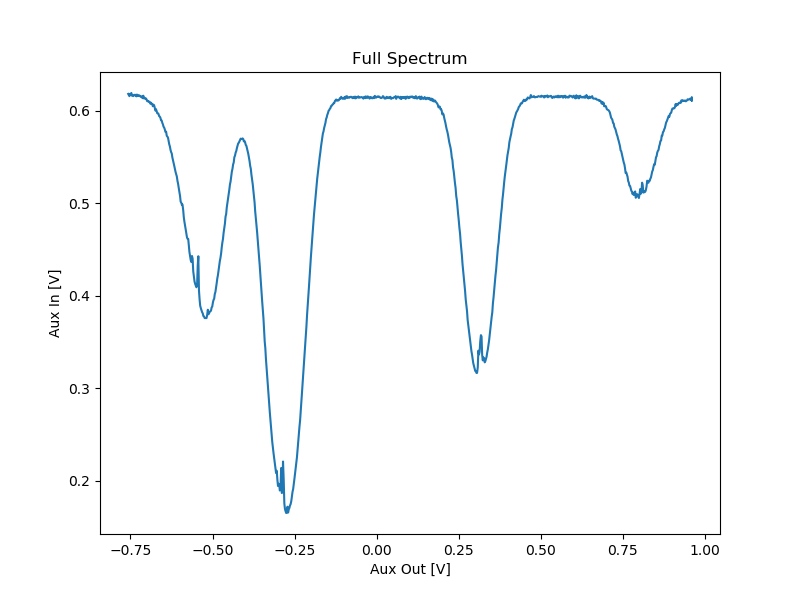
\includegraphics[width=0.5\textwidth]{fullspectrum.png}
    }
    \hfill
    \parbox{0.45\textwidth}{
        %\centering
        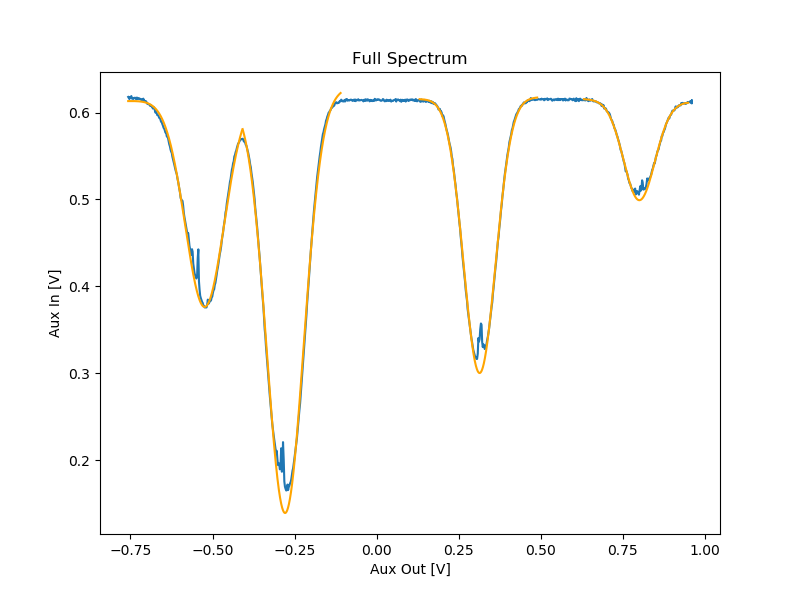
\includegraphics[width=0.5\textwidth]{fullspectrumgaussian}    
    }
    \caption{Left: Full Spectrum. Right: Gaussian Fits}
\end{figure}

Using the separations in $(\mu \pm \sigma)$ from one another, we can derive the calibration from the literature value of these separations. With the literature value\footnote{$= 6.8346826109042(90)\;\si{\giga\hertz}$\cite{script}} for the larger separation between Rubidium 87 $F = 1$ and $F = 2$, we can calculate

\begin{equation}
\alpha^{-1} \equiv \dv{V}{f} = (1.9366 \pm 0.0008) \cdot 10^{-10} \quad \si{\frac{\volt}{\hertz}}
\end{equation}

We then assume a linear proportionality $f \propto \alpha V$ and use $\alpha$ to convert any difference in volts $\Delta V$ to a difference in Hertz $\Delta f$:

\begin{equation}
\Delta f (\Delta V) = \alpha \Delta V
\label{conversion}
\end{equation}

Comparing the literature value of the separation in the Rubidium 85 $F = 2$ and $F = 3$ dips\footnote{$=3.0357324390(60) \;\si{\giga\hertz}$\cite{script}} with the one calculated from \autoref{conversion}, we can estimate an uncertainty in $\alpha$, which we found to be $(0.71 \pm 0.06) \%$. This is sufficiently accurate for the purposes of this experiment.

\subsubsection{Natural Transition Line Width and Doppler Broadening}

We then analysed the spectra we recorded for each individual Gaussian dip. Once again using \autoref{gaussianfit} as the fit function while masking out the Lorentzian peaks, we received a Gaussian profile which we could then subtract from the data in order to further analyse the Lorentzian peaks.

\begin{figure}
    \centering
    \parbox{0.45\textwidth}{
        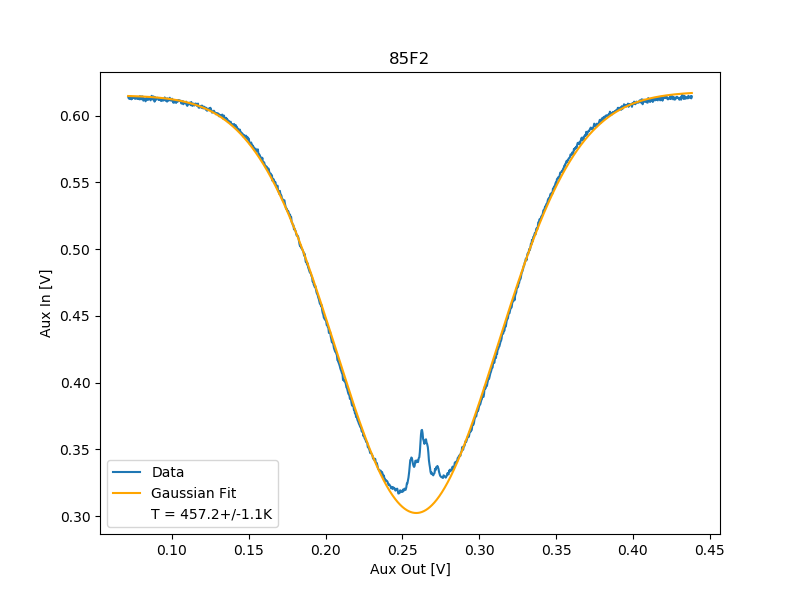
\includegraphics[width=0.5\textwidth]{gaussian1.png}
    }
    \hfill
    \parbox{0.45\textwidth}{
        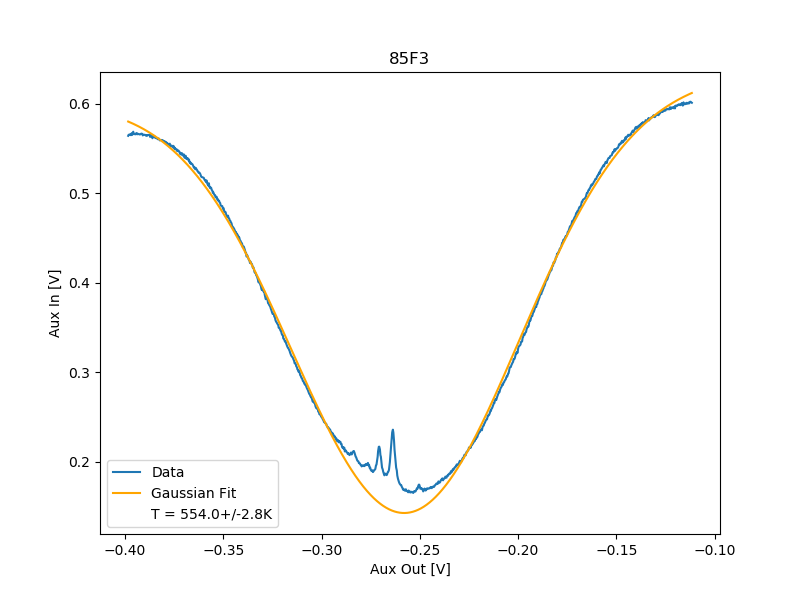
\includegraphics[width=0.5\textwidth]{gaussian2.png}
    }
    \parbox{0.45\textwidth}{
        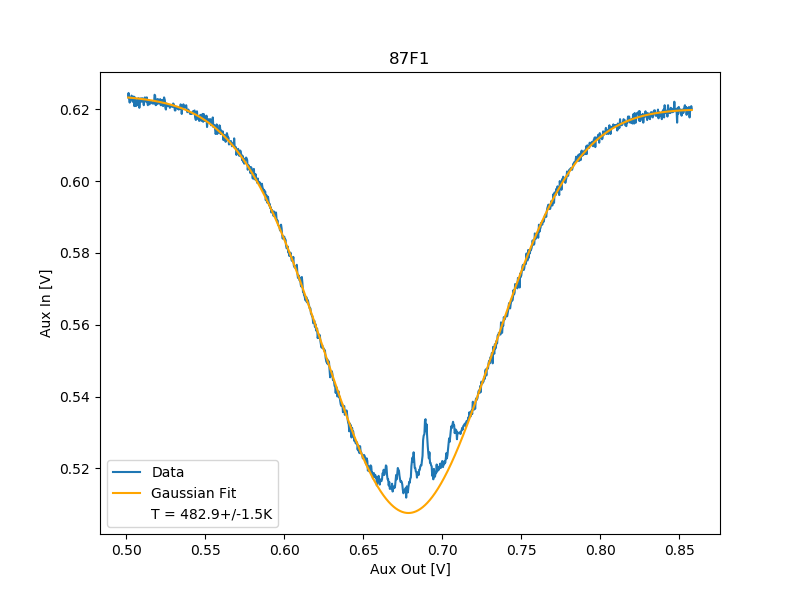
\includegraphics[width=0.5\textwidth]{gaussian3.png}
    }
    \hfill
    \parbox{0.45\textwidth}{
        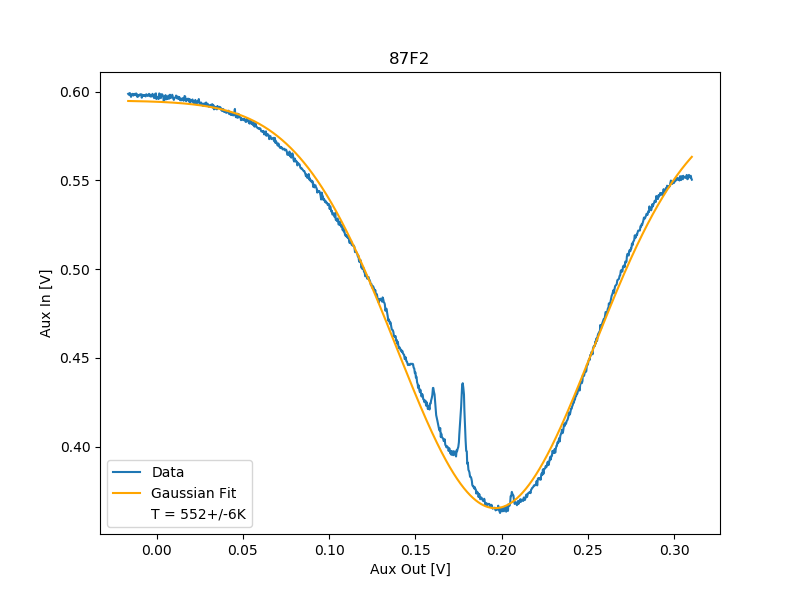
\includegraphics[width=0.5\textwidth]{gaussian4.png}
    }
    \caption{Gaussian Profiles}
    \label{gaussianprofiles}
\end{figure}

From the Standard Deviation of these Gaussian Profiles we can also calculate the temperature of the atomic sample:

\begin{equation}
T = \sigma^2 \frac{mc^2}{\nu_0^2 k_B}
\label{temperature}
\end{equation}

Where $m$ is the atomic mass of a single Rubidium atom, $c$ is the speed of light, $\nu_0 = \frac{c}{\lambda}$ is the laser frequency and $k_B$ is the Boltzmann constant. Since we are not yet cooling the sample, we would expect values around $300\si{\kelvin}$. The individual results are shown in \autoref{gaussianprofiles}.

Once we've subtracted the Gaussian from the data, we can fit a Lorentzian curve to each of the individual peaks:

\begin{equation}
A_0 \underbrace{\frac{1}{\pi\gamma}\frac{\gamma^2}{(x-x_0)^2 + \gamma^2}}_\text{Standard Lorentzian} + ax + b
\end{equation}

Where $A_0$, $\gamma$, $x_0$ and $a$ and $b$ are fit parameters. $\gamma$ is the scale parameter and $x_0$ is the location parameter, but we also added an amplitude $A_0$ to the Lorentzian to account for different peak heights. As before, $ax + b$ is a linear background function which accounts for both noise and peak overlap.

\begin{figure}
    \centering
    \parbox{0.45\textwidth}{
        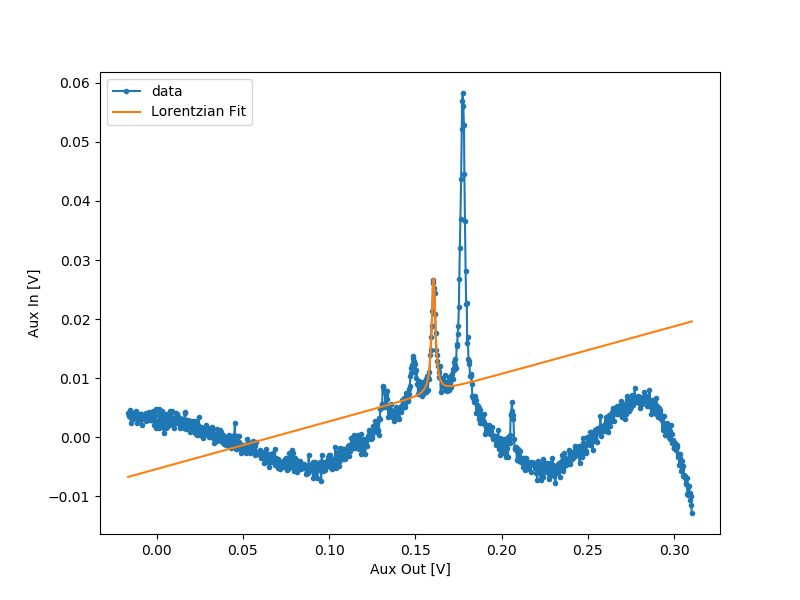
\includegraphics[width=0.5\textwidth]{lorentzianfull.png}
    }
    \hfill
    \parbox{0.45\textwidth}{
        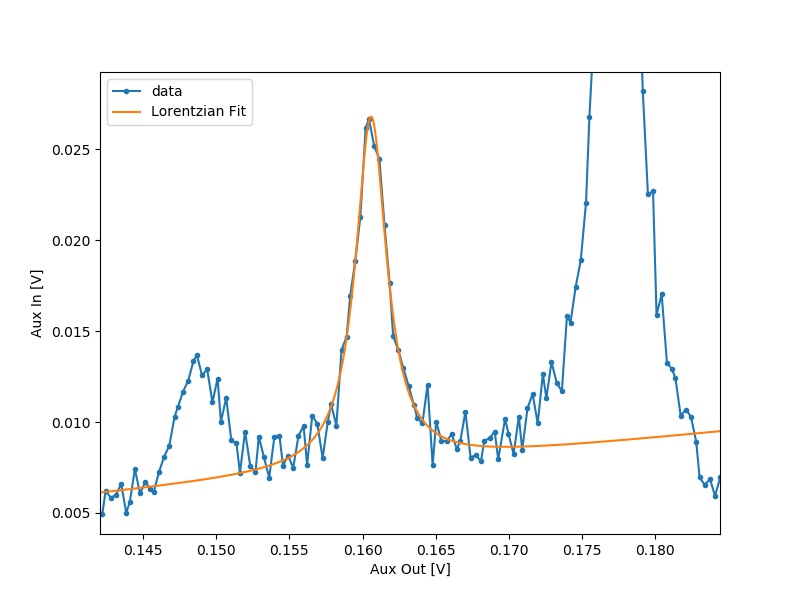
\includegraphics[width=0.5\textwidth]{examplelorentzian.png}
    }
    \caption{Full and Zoomed Lorentzian Profile and Fit For Rb 87 $F = 2$}
    \label{lorentzianprofile}
\end{figure}

Comparing the Natural Line Width $\gamma$ from the fits with the literature value $\gamma_{lit} \approx 6\si{\mega\hertz}$ \cite{script}, we receive the following values:

\begin{table}[htb]
\begin{center}
\caption{Lorentzian Fit Results}
\vspace{4mm}
\begin{tabular}{|c|c|c|c|}\hline
Isotope         & $F =$          & Fit Value in MHz   & Deviation from $\gamma_{lit}$ in $\sigma$ \\\hline
85              & 2              & $7.9 \pm 1.1$      & 1.7\\
85              & 2              & $13 \pm 4$         & 1.6\\
85              & 3              & $7.3 \pm 2.8$      & 0.5\\
85              & 3              & $7 \pm 4$          & 0.31\\
85              & 3              & $4.6 \pm 0.8$      & 1.8\\
87              & 1              & $9 \pm 4$          & 0.8\\
87              & 1              & $9 \pm 4$          & 0.8\\
87              & 1              & $11.0 \pm 1.2$     & 4.3\\
87              & 2              & $6.7 \pm 0.4$      & 1.7\\
87              & 2              & $5.3 \pm 0.8$      & 1.0\\\hline
\end{tabular}

\end{center}
\end{table}

Individual Lorentzian peaks for the same Isotope and energy level were considered from left to right. Note that not all peaks could be fitted due to the high SNR\footnote{Signal-to-Noise Ratio}.

\subsubsection{Hyperfine Splitting}

Lastly, we want to determine the hyperfine energy level separations of each Isotope and fine energy level. This means we need to assign each Lorentzian peak a hyperfine energy level and then calculate their mean distance. Since we also recorded the derivative of these spectra, we used that to determine the location of the peaks. To achieve this, we interpolated all neighboring points in each dataset with a linear function $f = ax + b$ and then solved $f$ for $0$ over the whole data range. Unfortunately, the SNR of these datasets was very high, on the order of up to $\approx 400\%$. To greatly reduce this, we introduced a rolling mean to each dataset, averaging over $20$ datapoints prior to interpolation. This reduced the overall SNR to $\approx 25\%$, which enabled us to solve $f$ at all, but introduces a statistical error in the solutions of $f$. This uncertainty can be estimated with the mean difference of data points on the (monotonically increasing) horizontal axis as well as the number of points we average over:
\begin{equation}
\Delta f_0 = N \cdot \frac{1}{n} \sum_{i = 1}^{n - 1} \left\lvert x_{i + 1} - x_i \right\rvert
\label{interpolationuncertainty}
\end{equation}
Where $f_0$ is a solution, $N = 20$ is the number of points averaged over and $n = 1000$ is the number of points in the dataset, with $x_i$ being the $i$-th point in the dataset.

\begin{figure}
    \centering
    \parbox{0.45\textwidth}{
        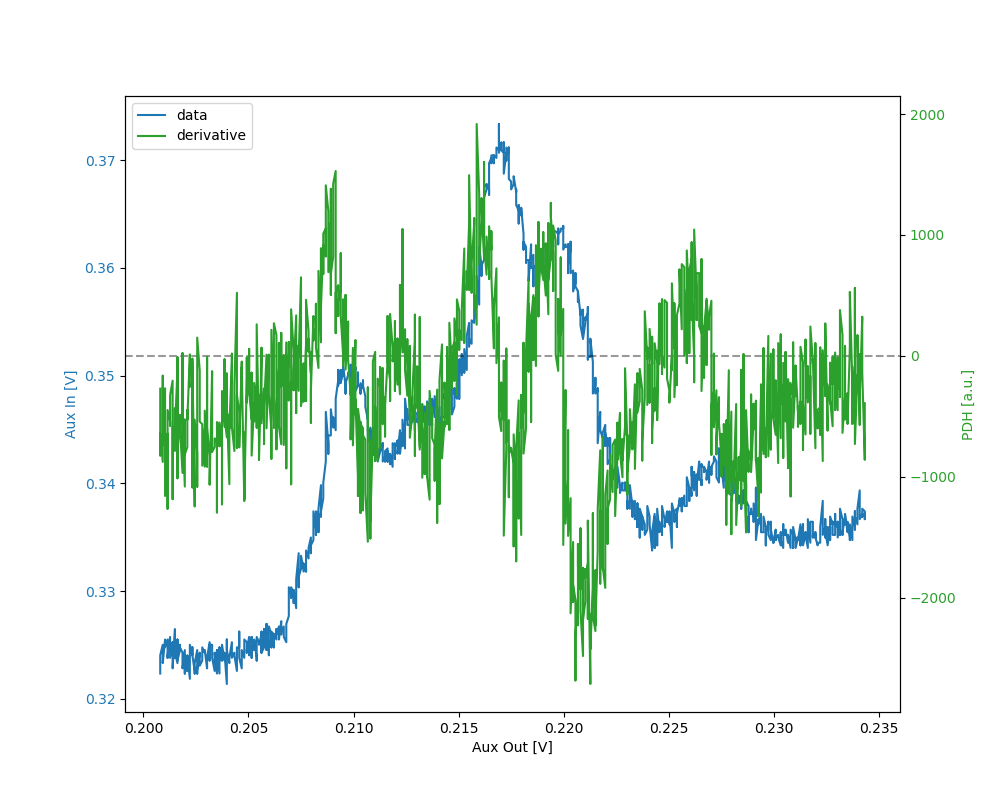
\includegraphics[width=0.5\textwidth]{originalderivative.png}
    }
    \hfill
    \parbox{0.45\textwidth}{
        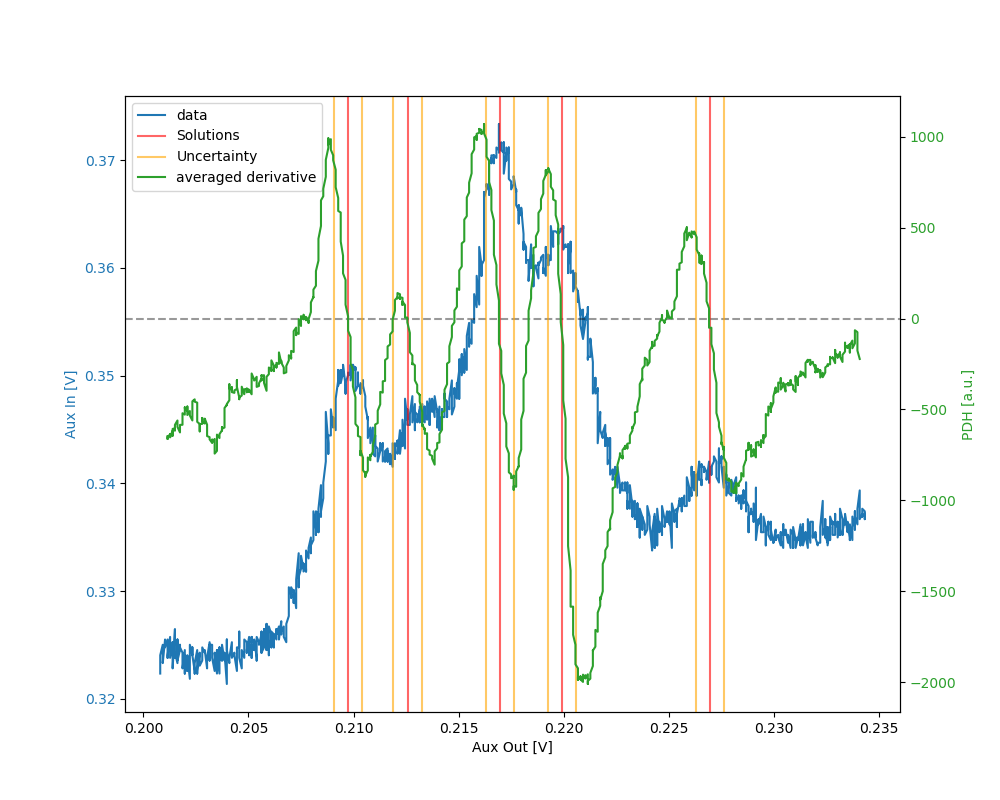
\includegraphics[width=0.5\textwidth]{averagedderivative.png}
    }
    \caption{Left: Signal with Original Derivative. Right: Signal with Averaged Derivative and Solutions}
    \label{lorentzianprofile}
\end{figure}

\begin{table}[htb]
\begin{center}
\caption{Hyperfine Separation Results\protect\footnotemark}
\vspace{4mm}
\begin{tabular}{|c|c|c|c|c|c|c|}\hline
Isotope     & $F =$  & $F'_1 =$   & $F'_2 =$   & Experimental Value [MHz]   & Literature Value [MHz]     & Deviation in $\sigma$ \\\hline
85          & 2      & 2          & 3          & $74 \pm 5$                 & $63.401(61)$               & 2.1\\
85          & 3      & 3          & 4          & $137 \pm 7$                & $120.640(68)$              & 2.3\\
87          & 1      & 0          & 1          & $92 \pm 10$                & $72.2180(40)$              & 2.0\\
87          & 1      & 1          & 2          & $131 \pm 10$               & $156.9470(70)$             & 2.6\\
87          & 1      & 0          & 2          & $223 \pm 10$               & $229.165(11)$              & 0.6\\
87          & 2      & 2          & 3          & $305 \pm 13$               & $266.6500(90)$             & 2.9\\\hline
\end{tabular}

\end{center}
\end{table}
\footnotetext{Literature Values taken from \cite{script}.}



\newpage

%%% LARS ENDE %%%

\subsection{Loading Curves}
\subsubsection{Generation of Loading Parameters, Optimisation of Loading Process}
The measurements as seen in Fig. \ref{examplemeas} (a) consisted of measured power meter voltage on the y-axis and time on the x-axis. In order to make use of these measurements, the voltage had to be converted into atom number (this rather complicated mathematical procedure shall only be mentioned here, the exact derivation can be found here \cite{script}). The loading curve with a subtracted background was then fitted to equation (7). This fit then allowed us to generate the parameters $\alpha$, $L$ and $N_{max}$ for varying detunings of the laser and currents through the anti-Helmholtz-coil. We then plotted these results in order to have an overwiev of the optimal parameters which generate the highest atom number and resolution (Fig. \ref{results_loading}). For completion, the magnetic gradient is calculated via:
\begin{equation}
\frac{dB}{dz}(z=\frac{R}{2})=1.1\times 10^{-6}\frac{NI}{R^2}
\end{equation}
where $R=8.5$ cm, $N=90$ windings and $I$ denotes the current through the coil.

\begin{figure}[h]
\centering
    \subfigure[$\alpha$ vs. detuning frequency for different currents]
{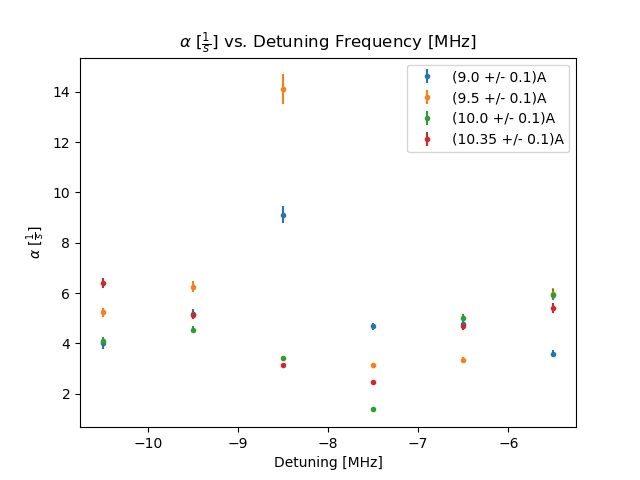
\includegraphics[width=0.4\textwidth]{alpha_gegen_det.png}}
    \subfigure[$L$ vs. detuning frequency for different currents]{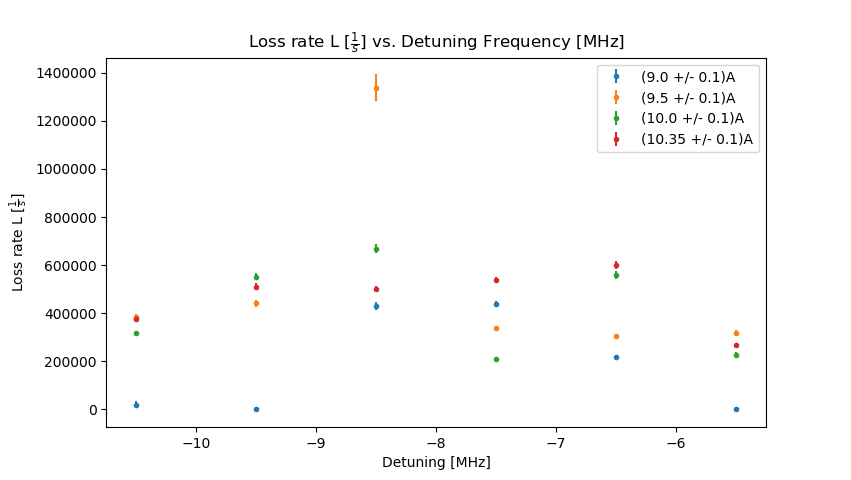
\includegraphics[width=0.5\textwidth]{loss_rate_gegen_det.png}}
    \subfigure[$N_{max}$ vs. detuning frequency for different currents]{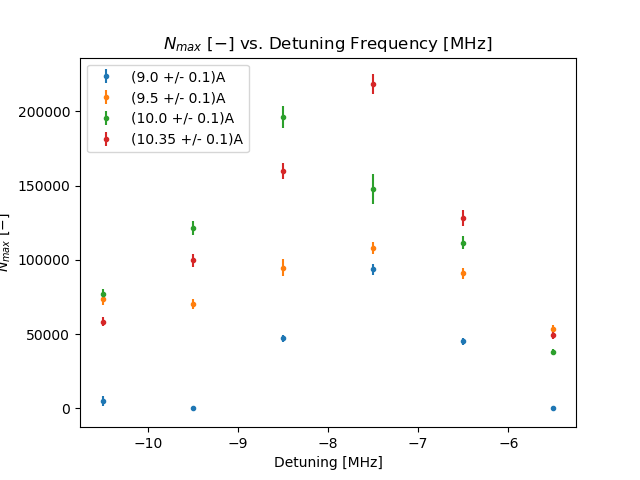
\includegraphics[width=0.4\textwidth]{particle_number_gegen_det.png}}
    \subfigure[3D plot: detuning vs. magnetic field gradient vs. $N_{max}$]{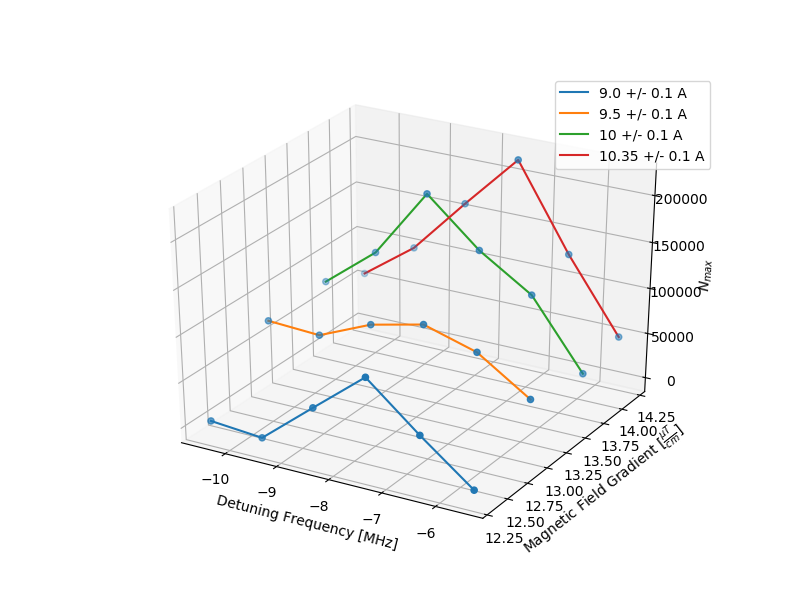
\includegraphics[width=0.5\textwidth]{3dplot.png}}
\caption{Results of 4.2.1}
	\label{results_loading}
\end{figure}
\newpage

As one can see: all parameters are highly dependent on the detuning of the laser and reach their maxima at about $-8.5$ MHz whereas a deviation from that value can lead to drops of  up to 60$\%$. During the experiment, we estimated a good set of parameters based on the intensity and size of the trapped atom cloud:

\bigskip
$f_{AOM}=(110.73 \pm 0.03)$ MHz (corresponds to a detuning of about $-8.5$ Mhz)

$I_{Anti-Helmholtz}=(10.00 \pm 0.05)$ A

$f_{AOM, spectroscopy}=2923.5$ MHz

\bigskip
Comparing this to Fig.\ref{results_loading}, one can see that these parameters generate the desired atom number and loading rates.

\subsubsection{Loading Curves and Calculation of MOT-Temperature}

\begin{figure}[h]
\centering
    \subfigure[equation (8) fitted to $\frac{N(t)}{N(0)}$ for varying shut-down times]
{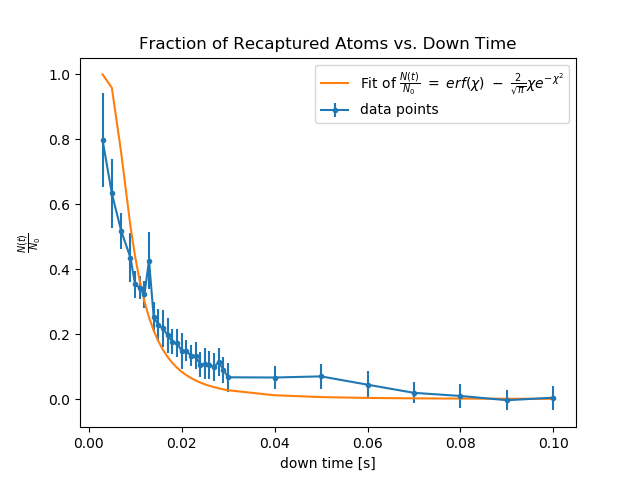
\includegraphics[width=0.45\textwidth]{erf_fit.png}}
    \subfigure[example of a loading curve used for the evaluation (9 ms down time)]{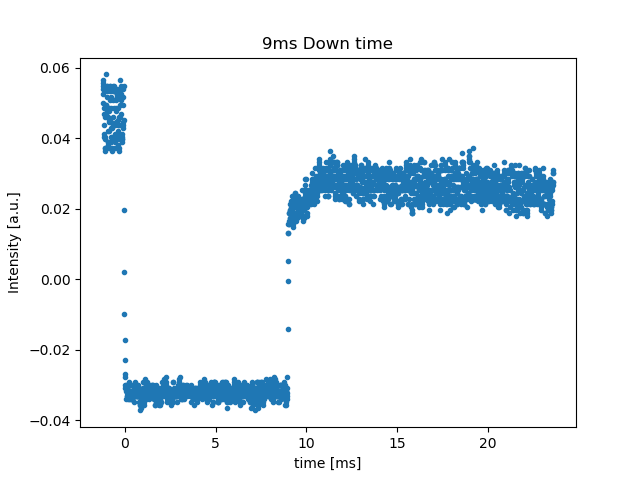
\includegraphics[width=0.45\textwidth]{9msdowntime.png}}
\caption{graphics concerning the calculation of the MOT-temperature}
	\label{erf_fit}
\end{figure}

The plot shown in \autoref{erf_fit} (a) was made using the curve-fit-module in
Python. The datapoints were generated by averaging over two time intervalls for
different down times: for example in \autoref{erf_fit} (b), we averaged over the
time intervall where the atom number was at a maximum and over the time period
right after the re-introduction of the laser beam at about 10 ms. These datapoints were then fitted to (8) in order to extract the temperature as a fit-patameter.

\bigskip
This method then yielded the following temperature for the trapped Rubidium atoms inside the MOT (with $M=85.4678$ u for the Rb-gas \cite{Rbmass})

\bigskip
\underline{$T_{MOT}= (225 \pm 16)$ $\mu$K}

\bigskip
which is right in the order of magnitude which we hoped to achieve (see 1.1.2).
Furthermore, the Fit has a $\chi^2_{red}$ of 2.8 showing that the model expressed by (8) does indeed describe the pyhsical subject accurately.






























%%% LARS ANFANG %%%

\newpage

\section{Discussion and Critical Analysis}

% regarding the temperature deviations from the gaussian profiles
\subsection{Spectroscopy}
\subsubsection{Multiplet Separation}
The calibration value $\alpha$ is sufficiently accurate for the purposes of the experiment. It is noteworthy that the background is not truly a linear function as we assumed here, but rather is caused by overlap of the 87F2 and 85F3 dips. It may be possible to achieve better accuracy through the use of another Gaussian background function, which would reflect the reality of the situation better.

\subsubsection{Natural Transition Line Width and Doppler Broadening}
While the temperatures we calculated are within the correct order of magnitude, their deviation from the expected $300\si{\kelvin}$ is quite large, suggesting that there is an underlying systematical uncertainty. Considering that the wider the range of the Lorentzian dips we had to mask is, the further the results stray from the expected value, we can assume that one of the most influential sources of this uncertainty is an inaccuracy in the fit. This is further confirmed by the fact that any uncertainty in $T$ stems purely from an uncertainty in $\sigma$ (with quadratic dependence), which is a fit parameter (see \autoref{temperature}). This method of calculating the temperature is perhaps better fit to be used on atomic samples in a different temperature range (such as close to absolute zero).

The Line Widths are all insignificantly different from the literature values, except for the final 87 $F = 1$ fit. Since we have a rather high SNR here, we can assume that this is the most influential source of any uncertainties which present themselves here. For these fits, it is imperative that the data points be very dense in the area of the fit, which was not necessarily achieved well here due to limitations in the lab equipment. Better fits and as such more accurate Line Widths could be produced by making more accurate measurements closer to the peaks as an additional measurement. Laser noise also plays a great role in these measurements.

\subsubsection{Hyperfine Splitting}
None of the evaluated separations deviate significantly from their respective literature values. The greatest source of uncertainty here is the SNR in the derivative. It might be possible to achieve better results through using the same method of rolling mean (with smaller N) and interpolation together with peak finding on the original dataset rather than the derivative, simply because its SNR is too high. That said, linear interpolation is, of course, an approximation of the real values and contributes to the uncertainty in these values. As shown in \autoref{interpolationuncertainty}, the uncertainty can be linear reciprocally reduced through increasing the density of the data points.
%%% LARS ENDE

\subsection{Loading Curves}
In the process of generating the loss rate and loading rate coefficients, we managed to keep the percental error rather low (Fig. \ref{results_loading}). Here, the error mostly stems from the high noise of our photodiode, which was set to maximum gain and the actual fit uncertainty (which is also related to the high noise). Therefore, the one way to maximise the accuracy would be to encapsulate the whole experiment into a light-sealed box with more sensitive photo diodes. This would in turn yield more accurate maximal atom numbers (or intensities) and thereby imoprove the fit of (8). However, the biggest error is induced by averaging over the intensities left and right of the down time valley as seen in Fig. \ref{erf_fit} (b). This introduces an error statistical in nature, which reduces the MOT-temperature accuracy to 7.1\%. These rather large statistical errors can be seen in \ref{erf_fit} (a), where the error is propagated to the fraction $\frac{N(t)}{N(0)}$, creating large uncertainties for fractions approaching 1. The release-recapture-method is thus limited by its statistical approach and the high noise of the photo diode mentioned above.

In conclusion this methods yields a surprisingly accurate result with 7.1\% uncertainty considering the experimentation was a rather quick process. However, the evaluation of 70+ CSV-data-files is a laborious process and maybe could be automated by a program, if this procedure were to be integrated into a scientist's working routine.


























\newpage 


%% Literatur)

\begin{thebibliography}{00}   % {00}: max 2-stellige Referenznummer
\bibitem{script} C. Hofmann, M. Repp, V. Gavryusev , S. H\"afner, \href{https://www.physi.uni-heidelberg.de/Forschung/QD/f20wikinew/index.php/Main_Page}{F20-Wiki}, Fortgeschrittenenpraktikum Heidelberg, Faculty for Physics, Heidelberg University
\bibitem{Rbmass} \href{https://physics.nist.gov/PhysRefData/Handbook/Tables/rubidiumtable1.htm}{NIST: Basic Atomic Spectroscopic Data}

\end{thebibliography}

\end{document}